%% It is just an empty TeX file.
%% Write your code here.
\chapter{Communication System Test}\label{ch:experiment}



\section {ParSec Communication System}
Various signals transmitted in industrial environment have different requirements in terms of dependability. Let's consider a simple CCTV video transmission system. Each frame, even in low resolution solutions, consists of several hundred thousands pixels. The frame rate lies somewhere between 30 and 5 frames per second, depending on the requirements. Even multiple bit error in the compressed video information bitstream leads just to the corruption of some frames. Depending on the error rate and frame rate, such disturbance may not influence the correct service at all, just lowering the video quality. The system, despite some errors, still fulfills it's function.

On the other hand the information flow between the control system and the nodes, placed on the robotic arms on the assembly line, consists in constant transmission of the coordinates of the destination and position of the arm. An error in such information can lead to the damage of manipulated objects or another catastrophic system failure.

Moreover, the quality of the signal propagation in such a rapidly changing environment is not constant. The error rate can significantly rise for a short time, but be relatively low otherwise. Spending time, power and resources on complex encoding and decoding may not be justified for the majority of the systems life time. The ability to adapt to the quality of the transmission would be just another advantage of well designed communication system.

In conclusion, the requirements of the industrial wireless system are diversified and need a configurable solution, that could offer a constantly high level of dependability while adapting to its environment and the use case. The high level of dependability means the coverage of the hardware faults in the first place, since they can even prevent the establishment and synchronization of the connection.

The goal of the ParSec project is to create a dependable, flexible and secure wireless communication system which meets all industrial automation requirements. It has to work with latencies below 1 ms and with very high noise level, serving many distributed clients at once. Moreover it has to deal with fading effects and potentially many reflections or even obstacles coming in the way of transmission and breaking it.

The ParSec communication system (shown in~\autoref{fig:ParSec}) consists of the MAC Layer processing, taking place within a standard processor, implemented mostly as software routines, followed by the a FEC unit and by a frame formatter. The last part is the baseband processor, which consists of mixed and analog signal processing and Radio Frequency unit. 

\begin{figure}[h]
\centering
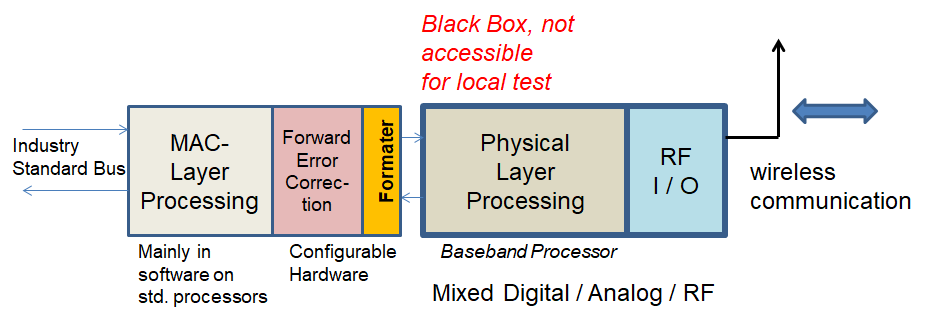
\includegraphics[width=0.65\textwidth]{figures/ParSec.png}
\caption{Block Diagram of the ParSec communiaction system}
\label{fig:ParSec}
\end{figure}

Both, the communication errors and soft errors due to transient faults in hardware, laying between FEC encoder and decoder, can be indifferently corrected thanks to ECC, as long as their number doesn't exceed the ECC correction capabilities. 

There are many techniques to improve the signal quality and make it resistant to fading effects due to multi-path signal propagation, poor signal-to-noise ratio or interferences, lowering the error rate. The known and used techniques involve Orthogonal Frequency Domain Multiplexing (OFDM) \cite{book:OFDM,art:OFDM}, Spread-Spectrum Communication \cite{art:spread-spectrum96,art:spread-spectrum97} or Ultra Wide-Band Frequency Communication \cite{book:ultra-wide08,book:ultra-wide04}. The OFDM technique would be suitable, but it ruquires many very fast AD converters~\cite{art:PSSS04}. The solution chosen for ParSec project is the Parallel Sequence Spread Spectrum (PSSS) technology~\cite{art:PSSS15,art:PSSS04,patent}. It provides comparable transmission quality as OFDM, without the cost of expensive AD converters.

The theory behind the creation of Error Correction Codes (ECC) has been presented in \autoref{sec:cod}. The detection and correction of single bit errors can be achieved using a simple Hamming code \cite{art:Hamming}. With Hsaio Code or extended Hamming Code the single error correction and double error detection is possible \cite{book:Fujiwara,art:Hsiao}. Unfortunately in such a noisy and harsh environment as industrial production site, there may be faults causing more than one or two bit flips in the data bit stream. For such purposes the multiple-bit correcting codes like Reed-Solomon code \cite{art:Reed-Solomon} or BCH Code \cite{art:BCH} are suggested. They typically require much more effort in  encoding and especially in decoding the information. They tend to be slower. There are also other methods to deal with correction of two-bit errors like \cite{art:Hosp, art:Varghese}. All these proposals lack a simple one-fits-all solution, that could be used and configured to the needs of the target system and it's environment.

The FEC in ParSec project is realized thanks to the Programmable Encoder Architecture (PENCA) designed by P. Pfeifer, firstly introduced in \cite{art:Pfeifer}, showed in~\autoref{fig:PENCA}. It is an answer to the strict requirements of the dependable communication systems. The core of the solution consists in the "honeycomb" structure of units. The units can be replaced by neighboring units in case of errors detected in one of them. The internal test can be performed automatically or on demand. After testing, the unit can be marked as faulty, once the test fails, and its functionality logically remapped into another unit. Both the input and output units are implemented in two copies, since they are single points of failure and in case of permanent fault detected wouldn't be able to get repaired without a spare. The control of the system is done through the microcode (secured with parity bits). But above all, the architecture can be configured to serve as different channel encoders, starting with the implementation of the single error correcting codes and ending with the multiple-bit error correcting codes or even cross-parity codes. It is done via generation of polynomials by each unit and sometimes even borrowing resources from neighboring units for more extended polynomial generations. Each unit being able to perform BCH generator polynomial length task up to 42 coefficients (34 BCH codes) or 65 coefficients (50 BCH codes) with borrowed resources.
 \begin{figure}[h]
 \centering
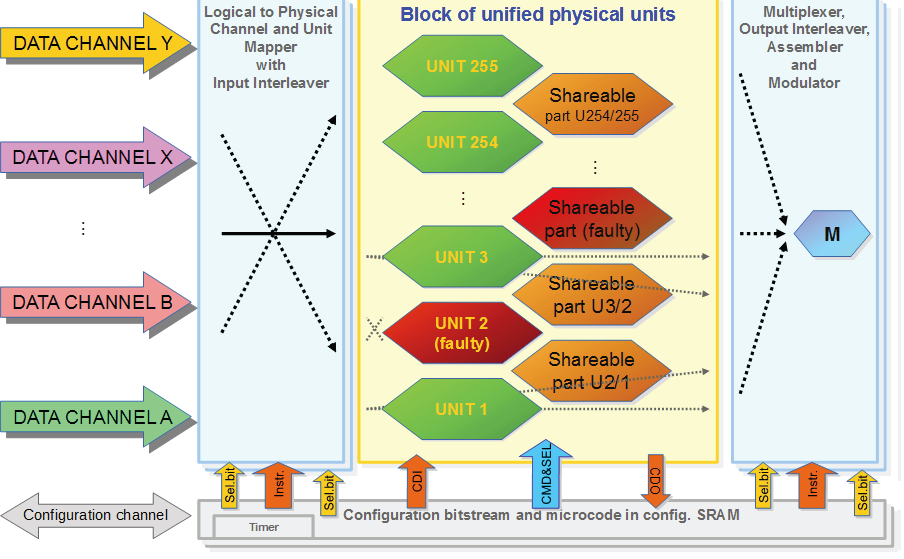
\includegraphics[width=0.65\textwidth]{figures/PENCA.png}
\caption{Basic scheme of the new dependable PENCA architecture~\cite{art:Pfeifer}}
\label{fig:PENCA}
\end{figure}

\section{Functional Shorts Concept}\label{sec:shorts}
The hard errors due to permanent faults in hardware modules require special treatment since they can even prevent the synchronization of transceiver and receiver and therefore cannot be so easily corrected by FEC. Since permanent faults don't disappear, they also need special repair mechanism, which often means a doubling of the unit or its parts. The fault diagnosis proves to be complicated, especially in the mixed signal and analog parts, moreover when the access to this parts is limited. When an IP is shipped as a "black box" and there is no possibility to implement any internal DfT techniques, some sort of external test is required. 

Thanks to the ECC, a precise detection of error positions in the received bit stream is possible, as long as the error count doesn't exceed ECCs correcting capabilities. The idea behind the diagnostic test based on extended FEC functions is to use the existing FEC redundancy and detect not only soft errors and transmission errors, but also hard errors due to permanent faults. As mentioned in the~\autoref{sub:limits} the ECC can be used in hardware monitoring only if the input and output of the UUT are identical. Since the wireless communication is usually a duplex communication, every node happens to own both, the transmitter and receiver. They consist of complementary building blocks. Every modulator in transmitter is substituted with a demodulator in receiver, every encoder with decoder. The basic task of the receiver modules is to recreate the original information sent by transmitter, step by step, layer by layer. A diagnostic test would require to short the transmitter with receiver and systematically short the outputs of every module with the inputs of their corresponding module. With encoder and decoder in one closed system, it should be possible to detect the exact positions of errors in the bitstream and identify faulty units. The decoder would act as a response analyzer. In this way, the information leaving FEC encoder arrives at the input of FEC decoder, manipulated only by permanent faults in the shorted modules. The idea is presented in~\autoref{fig:Shorts}. 

\begin{figure}[h]
\centering
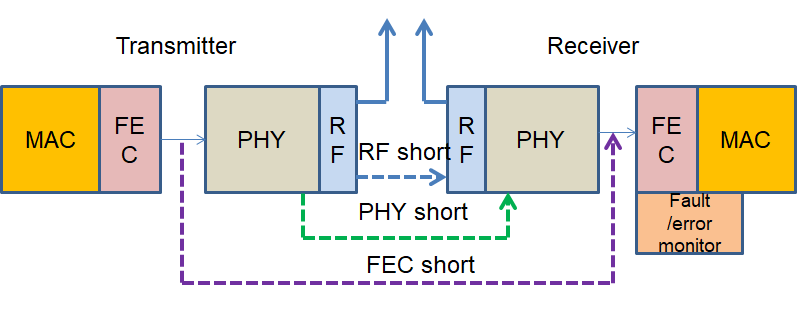
\includegraphics[width=0.65\textwidth]{figures/Shorts.png}
\caption{Transmitter and receiver shortcut idea for diagnostic test purposes}
\label{fig:Shorts}
\end{figure}

In order to conduct such test, the physical shorts need to be implemented. A simple multplexer demultiplexer pair with the common control logic would allow to choose between a normal functionality and shortened path. Additionally the test vectors need to be generated or stored in ROM. A good alternative would also be to do a "fake" start-up to detect all errors that may prevent the synchronization in advance. The test may be followed by random test to uncover other faults. The generation can happen even in software and be sent as normal information over the channel. The fault detection occurs thanks to an extended decoder functionality, which signalizes, with a special ISERR output, if the current bit of the bit stream has been flipped or not. This functionality is intended also to be used during the normal data flow, to adjust the transmission parameters and adapt the FEC algorithm. A simple counter connected to this special output counts the number of bit flips in every block. This information can be used for channel quality estimation, since the more errors per message, the worse is the transmission channel quality. 

The idea of functional shorts has been implemented into the Test Bench together with error injection capability and is shown in \autoref{fig:short_ena}. The injected error vector travels through the design together with test data. This guaranties the proper alignment of the error vector with the test vector at any time, also during the shortcut, when the path is shorter. It flips the specified bits of the output of any chosen module to simulate the possible effects of hardware faults on the processed information. The implementation lacks real modules, except for the encoder and decoder. Every other module is implemented as a simple delay in the digital information flow (flip flop) and XOR gate to conduct the error injection. They also have special enable signal to choose which module should occur as faulty. The enable signal is exclusive, meaning that only one module may be faulty at the same time. The Air simulates the communication channel. There is also a programmable delay to variate the execution time of the test and to simulate the fact, that the number of clock cycles, needed for the information to pass from the encoder to decoder, is not constant in all tests.

\begin{figure}[h]
\centering
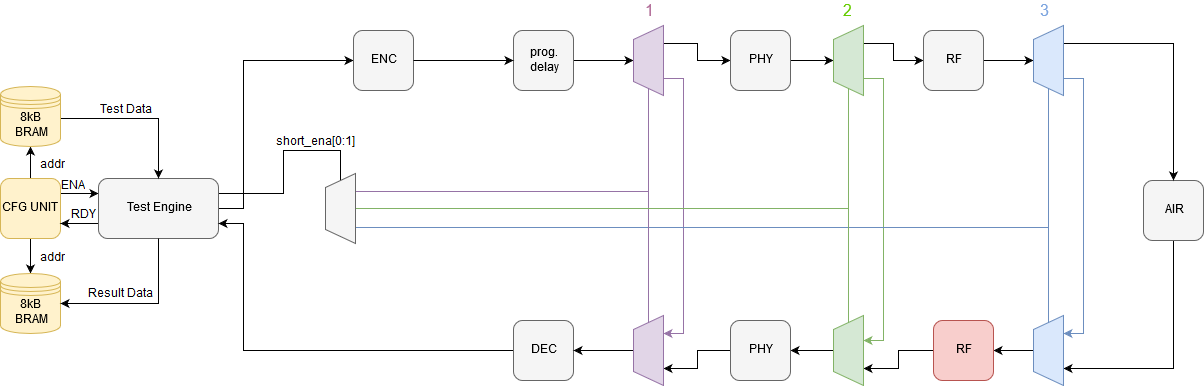
\includegraphics[width=\textwidth]{figures/Short_ena_err.png}
\caption{Implementation of functional shorts into the Test Bench}
\label{fig:short_ena}
\end{figure}

\subsection{Diagnostic test Procedure}
Let's assume, that the FEC decoder is fault-free and that every module owns some sort of repair ability. The erroneous unit would be the Radio Frequency unit of the receiver (marked red in \autoref{fig:short_ena}).
\begin{enumerate}
    \item Start the test by enabling the shortcut nr. 3, closing the test loop between transmitter and receiver, excluding all transmission errors from the test.
    \item Conduct the test by running all test vectors through the design, placing them on the inputs of FEC encoder, until the first occurrence of the ISERR output of the decoder module.
    \item Enable Shortcut nr. 2.
    \item Run test again and detect no errors, since the faulty unit is not in the test loop.
    \item Run repair procedure on the transmitter RF unit.
    \item Enable Shortcut nr. 3.
    \item Run the test only to see the ISERR is high again, because the repaired unit was not the faulty one.
    \item Run repair procedure on RF unit of the receiver, revert the repair of the transmitter RF unit.
    \item Start the test again to see no errors detected.
    \item Log the information about the repaired unit.
    \item Switch off all Shortcuts and start normal operation.
\end{enumerate}

After running the tests, all injected errors have been detected and the shorts system was able to identify the faulty unit. The number of injected faults have deliberately never exceeded the error correction capabilities of the decoder and the decoder was always assumed to be fault-free. Additionally the faults have been injected in random places, not necessarily corresponding to real permanent faults effects. Since the encoder and decoder are the only real modules in the test loop and their fault free functionality is crucial to the successful diagnostic test, they have been tested in isolated environment to understand their behavior and test their limits and possible impact on the whole system.

\section{Test of BCH(1023,943) Encoder}
The tested encoder is a BCH encoder taking 943 payload bits and calculating 80 parity bits. The encoder is actually a part of the PENCA architecture, without any redundant test and configuration circuitry. The encoder consists of an LFSR for parity calculations and the counter to keep track on the number of input user bits. Before the counter reaches 943 bits, it forwards the user bits to the output. Then the parities are shifted out with "dummy" input bits. The parity calculation is obtained by dividing the input polynomial by the generator polynomial of the encoder. The rest of the division is the parity polynomial. The general architecture of a BCH encoder using a LFSR for polynomial division is shown in \autoref{fig:enc_0}. Since the test bench developed during the project allows a test with wide range of frequencies, it may be possible to cause some delay faults in th encoder architecture and examine, how they influence the output bit stream.

\begin{figure}[h]
\centering
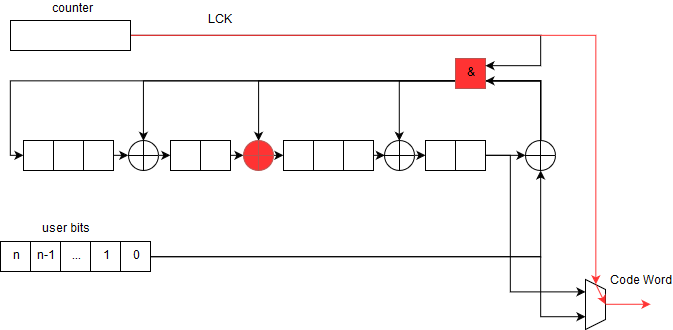
\includegraphics[width=0.65\textwidth]{figures/BCH_ENC.png}
\caption{A BCH encoder architecture \cite{art:BCH_implement}}
\label{fig:enc_0}
\end{figure}

The encoder has been placed in the test bench and tested for maximum frequency. The input data is random. There were 300 messages sent and evaluated. The comparison data was calculated using MATLAB 2015b comm.BCHEncoder. There were two encoder versions tested. One version is surrounded by flip-flops to guarantee that the delay fault happens in the encoder design and not due to the long connection paths between encoder design and the test Engine. This version was called "isolated". The "not isolated" one was connected simply to the input and output registers of the test bench. The results are shown in \autoref{tab:enc}.

\begin{table}[h]
\begin{tabular}{@{}lllll@{}}
\toprule
UUT                       &mem\_width   &uut\_width &expected freq. &max. freq.\\ 
\midrule
isolated Encoder                  & 32          & 4      & $\sim$642 MHz & $\sim$500 MHz \\
not isolated Encoder              & 32          & 4      & $\sim$642 MHz & $\sim$326 MHz \\
\bottomrule
\end{tabular}
\centering
\caption{Test Encoder for max. frequency}\label{tab:enc}
\end{table}

The result shows clearly, that a Test Engine limit has been reached while testing the isolated Encoder. The not-isolated version is failing due to long interconnects. Though the triggered delay fault did not happen in the internal structure, 
it simulates the effect of the transition delay fault in one of the gates connected directly to the input or output registers of the test bench. The further analysis can reveal which gate would that be and how many bits were changed.

The Encoder test was conducted with random data input. First clock cycle is reserved for the reset. When the reset is low, the input vector is shifted in serially. The output is equal to the input when the payload bits are shifted in. After 943 payload bits, the input is set to zero and held that way till the end of the test, which means another 80 clock cycles for the parity bits to be shifted out. 

\autoref{fig:enc_1} represents the result of the failed test at approx. 355 MHz. Only parity bits are visible, since the errors happened there. The Y-Axis shows the number of the failed massage and the X-Axis represents the number of the bit that failed. In half of the messages the first parity bit is corrupted. When the counter, calculating the number of shifted bits, reaches the 943, the output should be switched to the parity bits (see \autoref{fig:enc_0}). In all vectors, the output still forwards the input value, which is zero for all "dummy" bits. In half of the vectors, since they are randomly distributed, the zero is accidentally the expected value, therefore the error gets masked.

The raised frequency, together with very long interconnect simulated a fault in the multiplexer, which does not react to the select signal fast enough or in the logic producing the delayed select signal. The outcome is a single bit error.

\begin{figure}[h]
\centering
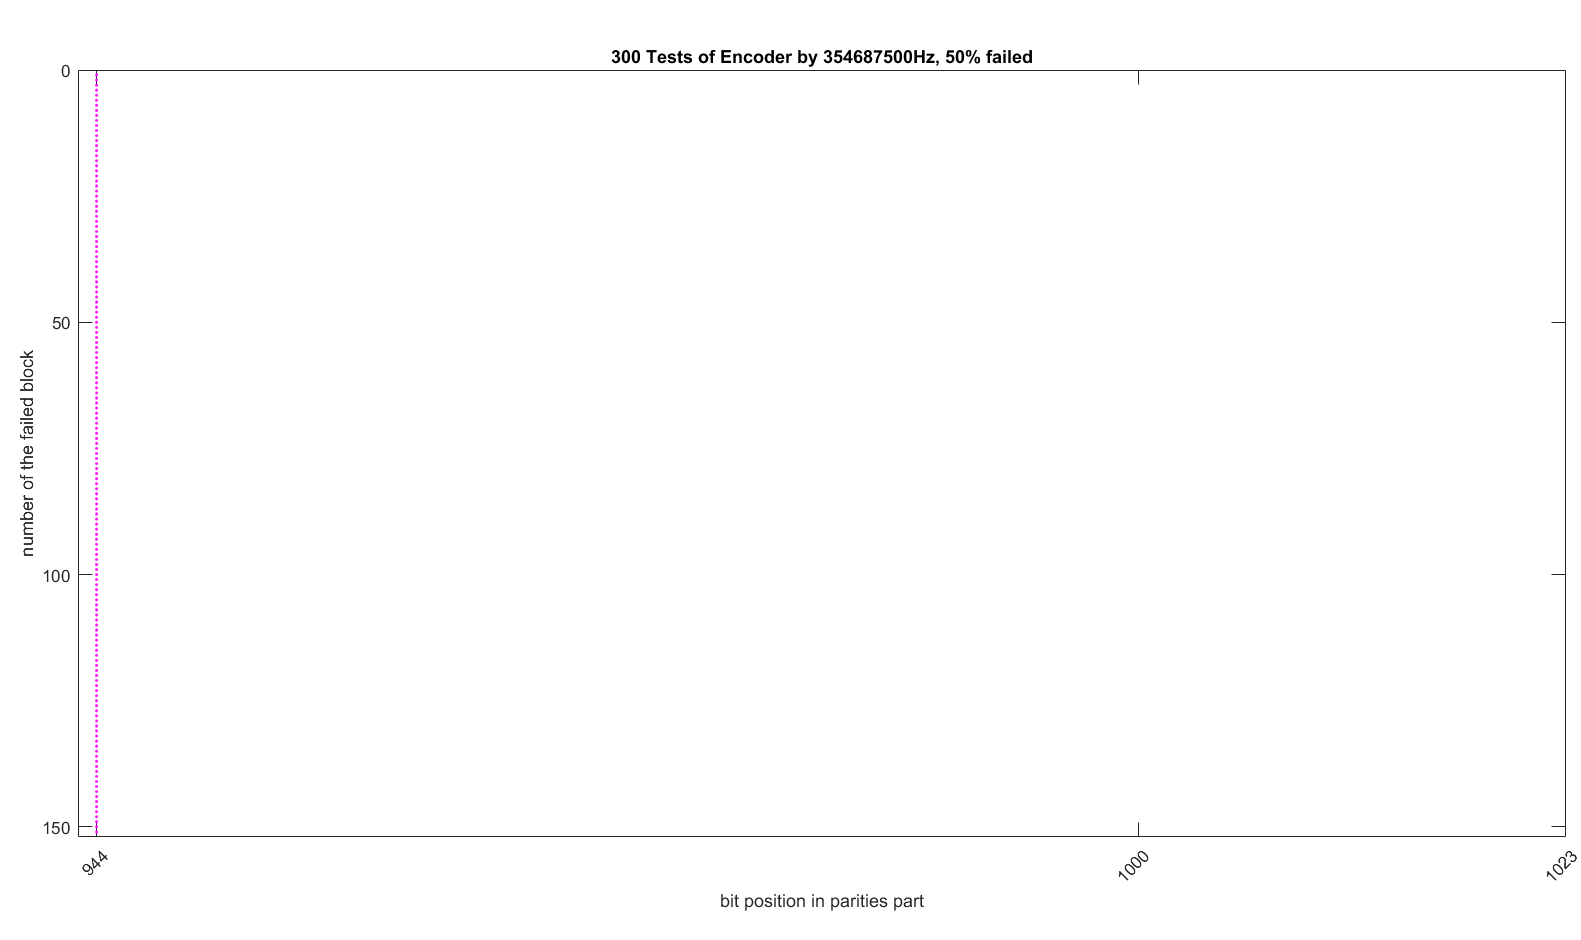
\includegraphics[width=\textwidth]{figures/test_ENC_1.png}
\caption{The result of failed Encoder test by 355 MHz}
\label{fig:enc_1}
\end{figure}

The further raise of the test frequency reveals another path failing. The \autoref{fig:enc_2} shows the parity bits of the failed test. In addition to the 944th bit, there are more bits flipped in the parity part of the message. There is no possibility, that the LFSR would fail at such low frequency. The values from correctly calculated parity bits don't reach the input registers of the test engine within the time frame. The same effect would be visible if the permanent fault happened in the LFSR logic or on the input of the multiplexer, causing multiple errors in the parity bits. The serial structure of the encoder makes it more vulnerable against multiple bit flips due to permanent faults, since all bits need to pass the same hardware elements.

\begin{figure}[h]
\centering
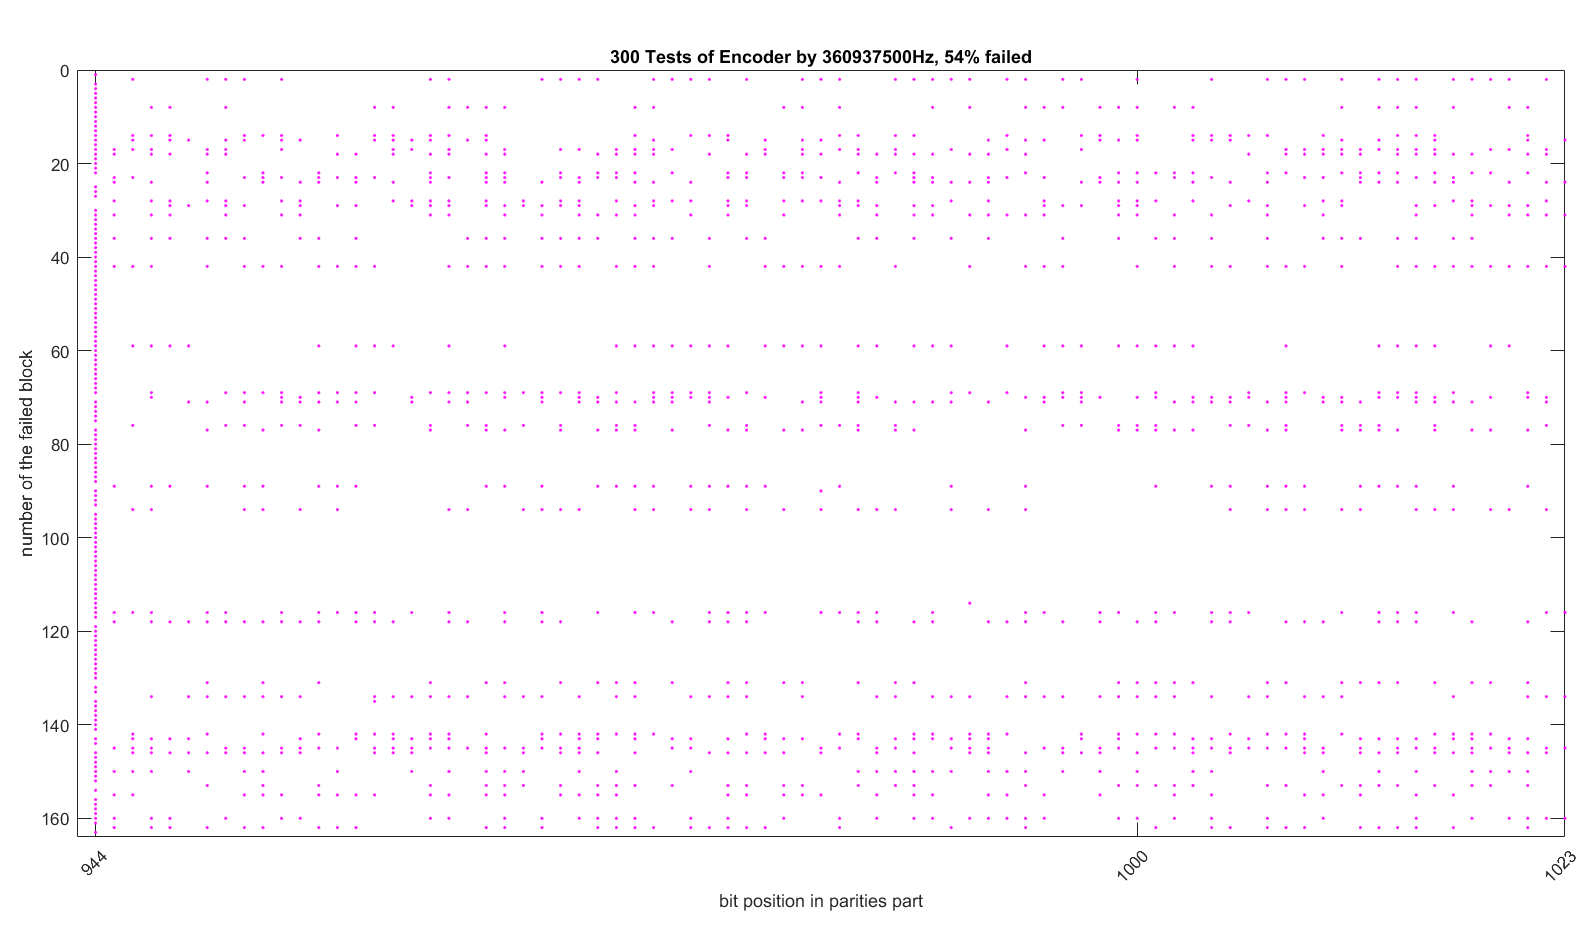
\includegraphics[width=\textwidth]{figures/test_ENC_multiple.png}
\caption{The result of failed Encoder test by 360 MHz}
\label{fig:enc_2}
\end{figure}

There are also examples from different encoder architectures, where despite their fast, parallel parity calculation, within one clock cycle, multiple bit errors are possible. It has been reported in \cite{art:Dicorato}, based on Hsiao-Code encoder architecture. The cause of the error are faulty XOR gates with big fan-outs, taking part in computation of more then one parity bit. The suggested solution involves the use of more XOR gates, making the design more regular to avoid big fan-outs. The regularity allows even additional self test and self repair functionality. This solution does not apply to the encoders with polynomial division architecture. But the usage of LFSR can be of advantage in different way. The LFSR is filled at the beginning with a starting seeding pattern as normal shift register. After running for a sequence of length k, the state of the LFSR in (k+1) tact should be equal to its initial state. The comparison of the seeding pattern and actual value, with simple XOR operations, would reveal any permanent fault in the LFSR. This self test may be used in any architecture introducing LFSR, like BCH encoder, decoder or PSSS bit spreading hardware\cite{art:Gleichner}.

Although the test results did not help in estimation of the maximal frequency of the encoder, they simulated some delay fault effects, which could have happened in real hardware. They showed a vulnerability of encoders with serial and long parity generation, resulting in multiple error bits, which may possibly not be detected by the diagnostic test, due to their number going far beyond any reasonable decoder detection capabilities.

\section{Test of BCH(1023,943) Decoder}
For any positive integers $m \geq 3$ and $t<2^{m-1}$ there exists a binary BCH code with the following parameters \cite{art:BCH_implement}:
\begin{subequations}
\begin{align}
    \text{block length }n&=2^{m}-1\label{eq:blck_len}\\
    \text{parity bits }k&\geq n+mt\label{eq:parity}\\
    \text{hamming distance }d&\geq2t+1\label{eq:dmin}
\end{align}
\end{subequations}
The BCH(1023,943) with its $n = 1023$ and $k=943$, has a $d_{min}= 17$. The code is therefore capable of detecting 16 error bits and correcting 8 in a single block. 

The tested BCH decoder has one serial data input (DIN) and one data output (DOUT). The input data enters the syndrome computation block, which is, similar to encoder, implemented as LFSRs. It is actually less complicated then the encoder, having shorter LFSRs to compute partial syndromes, one for every correctable error. When all syndromes are equal zero, the received message is a valid code word. In other case, when any syndrome is non-zero, the Key Equation Solver has to find the parameters of error locating polynomial. The parameters are passed to Chien Search Block to find the roots of the error locator polynomial and therefore the exact positions of errors in the received message. The output of the Chien Search Block is connected to the output ISERR to indicate, that the current output bit, has been repaired. To obtain the number of errors corrected, a simple counter connected to ISERR output is enough. It should be reseted with every new message. The decoder needs 97 clock cycles before it starts shifting out the corrected Code Word. The basic idea of building a BCH Decoder is shown in \autoref{fig:dec_0}.

\begin{figure}[h]
\centering
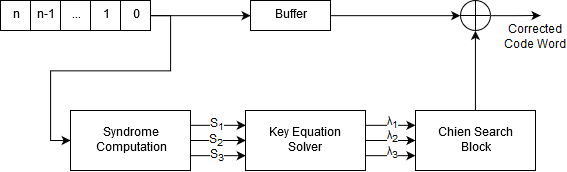
\includegraphics[width=0.65\textwidth]{figures/BCH_DEC.png}
\caption{A BCH decoder architecture \cite{art:BCH_implement}}
\label{fig:dec_0}
\end{figure}


The \autoref{fig:dec_1} shows a result of a simple test, where randomly generated data was "XORed" with randomly generated error vectors with raising hamming weight. Each test consists of 1000 messages and the error number is raised from 1 to 18. The decoder successfully detects and corrects all errors in those messages, where the number of errors does not exceed 8. It fails to detect any higher number of errors, giving a detection rate lower then 40\%. A successful detection does not mean, that all errors were detected, it only means, that the decoder signaled that there was any correction in the message, setting ISERR output at least once to 1.  The inability of error detection up to 16 bits shows, that the decoder was implemented only for error correction purposes and does not present the full functionality of the underlaying code. The decoders used in a communication with no time for retransmission, have to be able to correct as many errors as possible. If the error count exceeds its capabilities, there are two options. The message is accepted as fault free if the error vector transformed the original code word into another valid code word or the message is treated as faulty and repaired, resulting in wrongly decoded message. In either way, the received message is wrong. There is also a third option resulting from not perfectly distributed code words in the code space. The \autoref{eq:dmin} is an inequality for all not perfect codes. The perfect codes have equal distances between all code words. If the received message falls into the space where the decoder cannot unambiguously ascribe it to any code word, a special indication of failed correction should be possible. Faults detected by the decoder are due to wrongly corrected messages. The not detected ones were either valid code words or code words from outside the error correction spheres.

\begin{figure}[h]
\centering
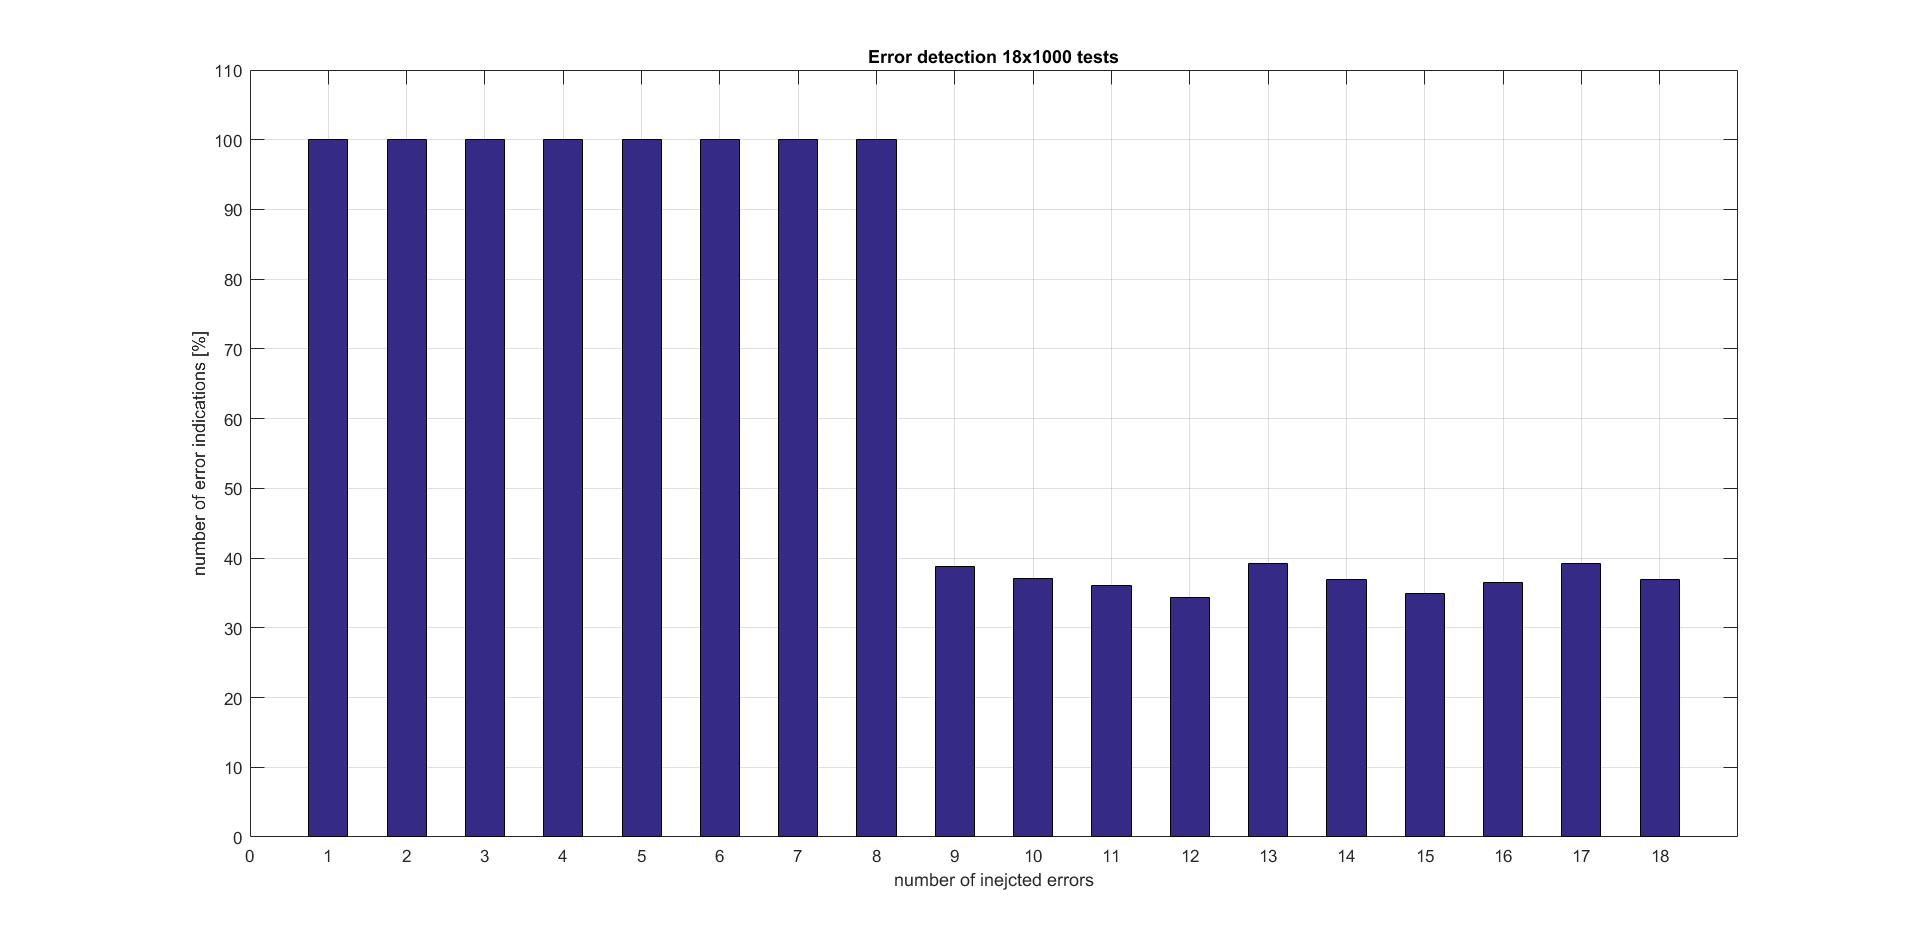
\includegraphics[width=\textwidth]{figures/1000_tests_error_detection.png}
\caption{The error detection limits of the decoder}
\label{fig:dec_1}
\end{figure}

\subsection{Test Decoder for maximal frequency}

The test procedure involving functional shortcuts assumed a fault free functionality of the decoder. It is possible though, that the decoder suffers from any permanent fault itself, giving false negative or false positive results of the test, not mentioning the problems during communication. The decoder was tested for its maximal operational frequency and beyond. The cut-off frequency depends on the number of injected errors. The decoder was tested only till its maximal detection capabilities, since there is no way to evaluate its correct response for more than 8 errors. The isolated version means again a design surrounded by flip-flops. The direct input and output is always compared with their delayed pairs to check, if the delay fault did not happen on the interface with test bench. The unconstrained design was tested first, allowing the tool to automatically place the design in the FPGA. The results are presented in \autoref{tab:dec}.

\begin{table}[h]
\begin{tabular}{@{}ccccll@{}}
\toprule
UUT                       &mem\_width   &uut\_width &error cnt. &\begin{tabular}{@{}c@{}}unconstrained \\max. freq.\end{tabular} &\begin{tabular}{@{}c@{}}constrained \\max. freq.\end{tabular}\\ 
\midrule
\multirow{9}{*}{\begin{tabular}{@{}c@{}}isolated \\Decoder\end{tabular}}    & \multirow{9}{*}{32}        & \multirow{9}{*}{8}       &0           & $\sim$264 MHz & $\sim$319 MHz \\
                            &                           &                           &1          &   $\sim$237 MHz &   $\sim$229 MHz\\
                            &                           &                           &2          &   $\sim$200 MHz &   $\sim$221 MHz\\
                            &                           &                           &3          &   $\sim$200 MHz &   $\sim$219 MHz\\
                            &                           &                           &4          &   $\sim$200 MHz &   $\sim$219 MHz\\
                            &                           &                           &5          &   $\sim$180 MHz &   $\sim$218 MHz\\          
                            &                           &                           &6          &   $\sim$160 MHz &   $\sim$219 MHz\\
                            &                           &                           &7          &   $\sim$160 MHz &   $\sim$218 MHz\\
                            &                           &                           &8          &   $\sim$160 MHz &   $\sim$219 MHz\\
\bottomrule
\end{tabular}
\centering
\caption{Test Decoder for max. frequency}\label{tab:dec}
\end{table}

The XML file returned by the test engine allows to examine the failed tests and see where the errors occur and in what number. The result evaluation of the test with 1 induced error is showed in \autoref{fig:dec_3}. There are 1000 messages to be corrected and the frequency is just above the limit, tacting the design with 238 MHz. The right-hand side graph shows the total number of errors resulting from overtacting. Their colors correspond to the type of output. They should be equal at all times, since the only way to flip the DOUT bit should be through the ISERR bit. The left-hand side graph represents all erroneous messages and the positions of errors. Dots represent the errors in the DOUT signal, the rectangles - errors in ISERR signal. The diamonds symbolize the positions of injected errors.

\begin{figure}[h]
\centering
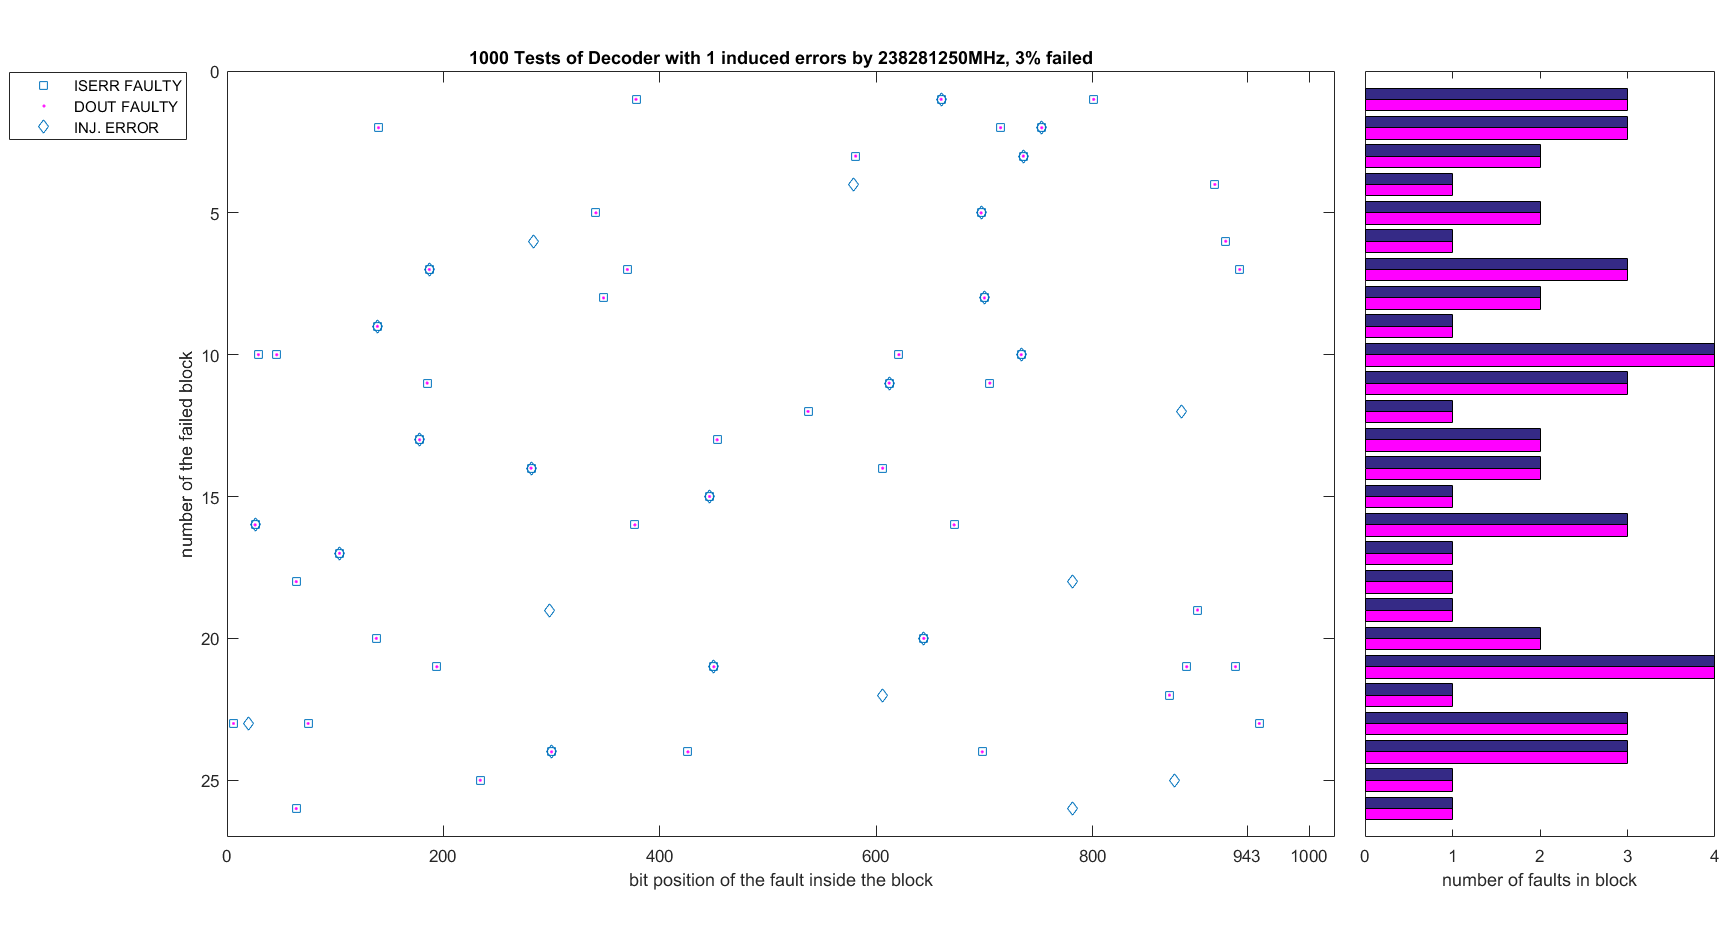
\includegraphics[width=\textwidth]{figures/1000_tests_1_faults_238_MHz.png}
\caption{Test of BCH Decoder with 1 injected error over its max. frequency}
\label{fig:dec_3}
\end{figure}

When the diamond marker is present without other markers it means, that the error was injected in this position and it was detected and corrected successfully. There are two types of errors. When all three markers reside in one position it means, that there was an error injected in this position and it was expected to be detected and corrected. The detection did not happen, therefore it was not corrected, causing an error both in ISERR and DOUT. All other cases are errors that got wrongly detected and corrected although none were injected in those positions - errors induced by decoder itself, marked as rectangle with dot. 

The error distribution is random, data dependent. The single syndrome computation is very similar to the parity computation in the encoder, since it also involves LFSR. The encoder test revealed, that it doesn't fail at such low frequency, hence the errors are produced somewhere in the Key Solver or Chien Search Block. If the Chien Search Block failed, it could produce more errors, then the theoretical decoder correction capability. Such thing was not visible during any of the tests. The fault is therefore probably in the Key Solver or control logic.

\begin{figure}[h]
\centering
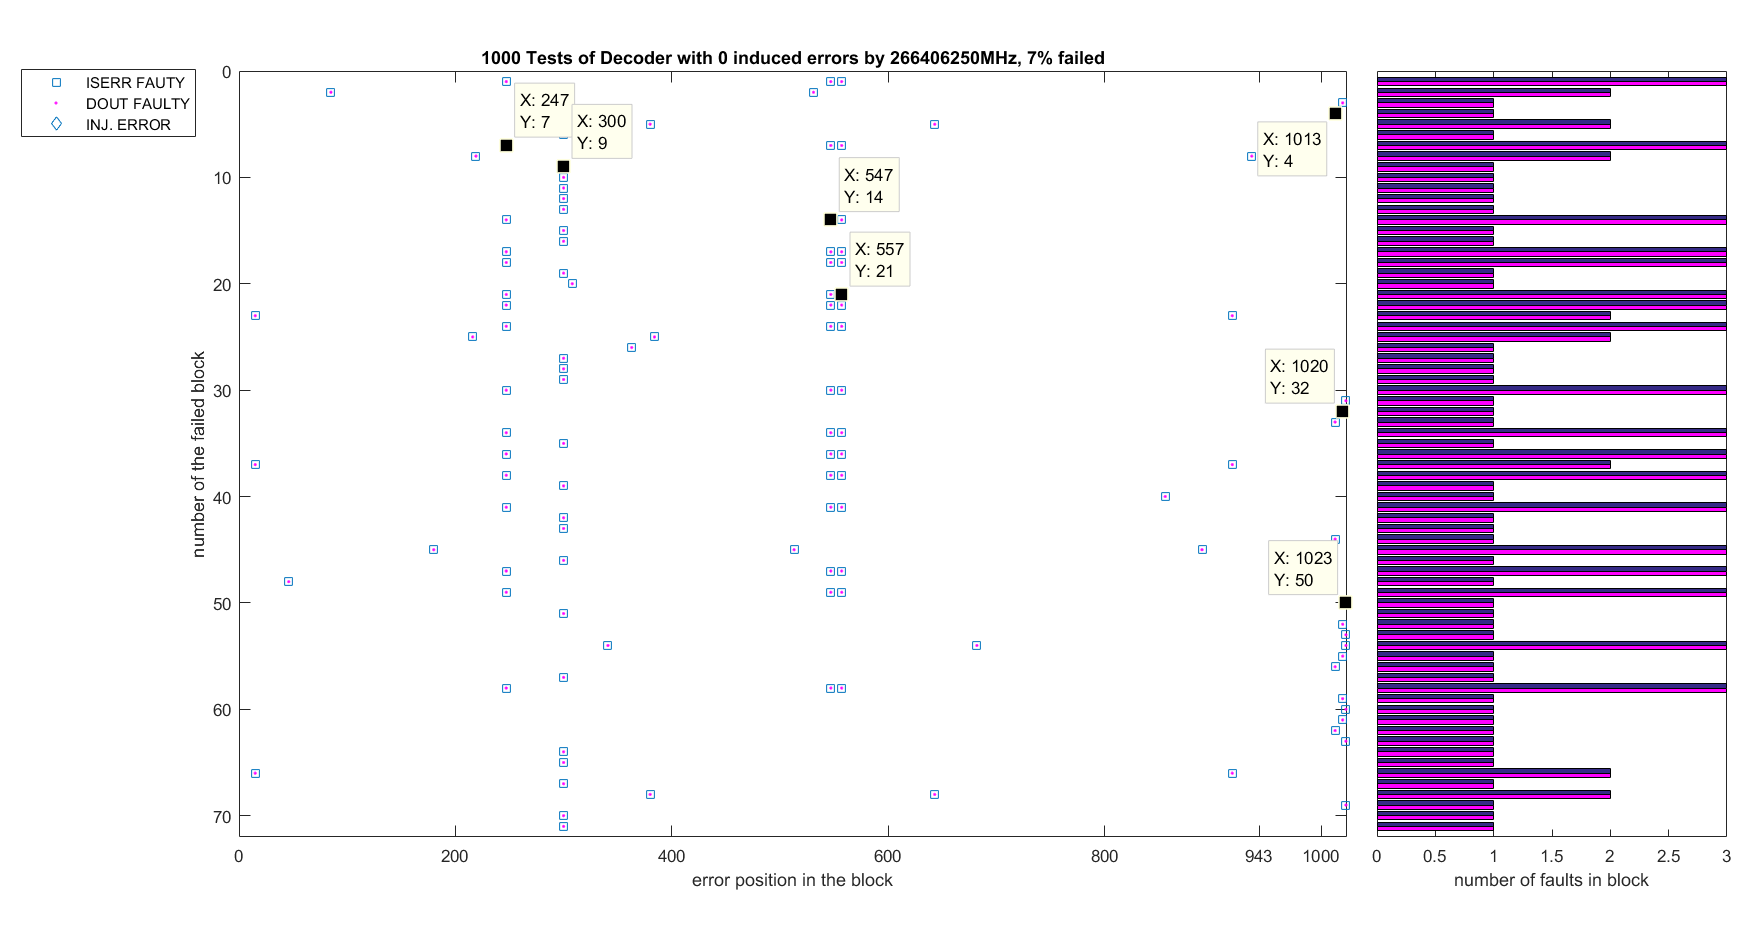
\includegraphics[width=\textwidth]{figures/1000_tests_0_faults_266_MHz_1.png}
\caption{Test of BCH Decoder with 0 injected errors over its max. frequency}
\label{fig:dec_2}
\end{figure}

In the test with no injected errors (\autoref{fig:dec_2}), the syndromes and therefore the parameters of error locator polynomial should be zero at all times. The error positions are not any more data dependent and random, but they occupy mostly the same positions throughout all failed tests. Again the suspected module is the Key Solver.

When the frequency gets closer to 300 MHz another characteristic errors appear in the decoder architecture. At first the result, analyzed as all others, showed a failure of almost all DOUT bits. The plot of this result represents no information at all. In the raw data, it was but visible, that the response signals are somewhat shifted in relation to the expected values. Again a cross-correlation function came to aid and allowed to determine the shift, which is equal $2$. The received signal needs to be shifted by $-2$ (2 to the left) to be aligned with expected signal. The result of the comparison after the shift is shown in \autoref{fig:dec_4}. 

\begin{figure}[h]
\centering
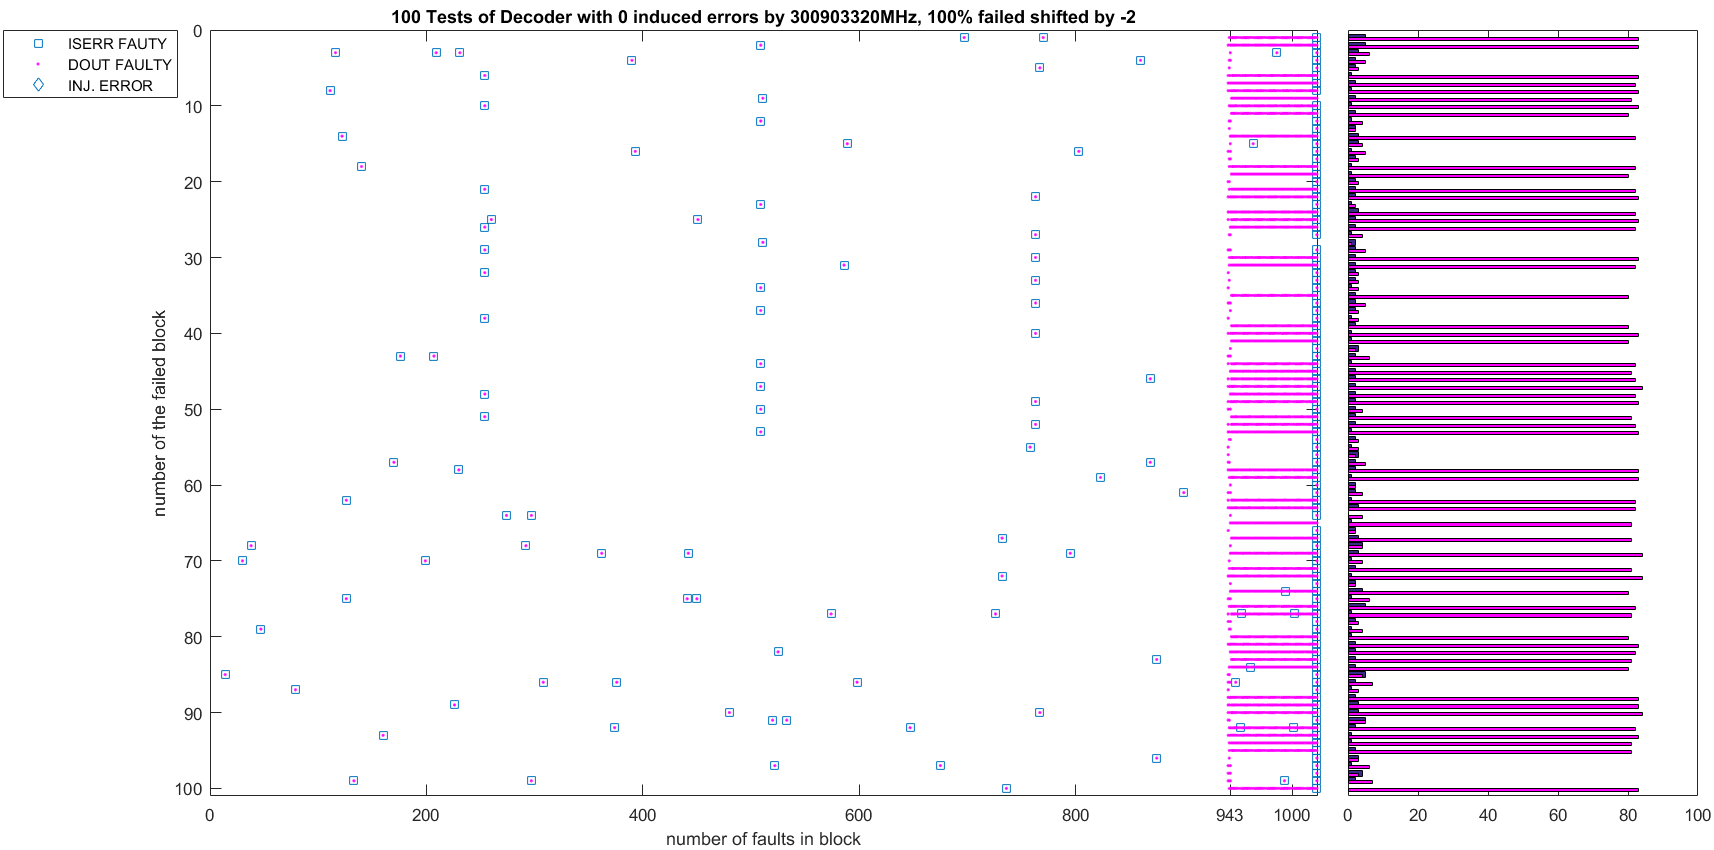
\includegraphics[width=\textwidth]{figures/100_tests_0_faults_300_MHz_shift_2.png}
\caption{Test of BCH Decoder with 0 injected error much over its max. frequency}
\label{fig:dec_4}
\end{figure}

The number of $ISERR$ errors is different then the number of $DOUT$ errors, which means that the error correction logic is not responsible for the wrong output. The further inspection reveals, that the value of 940th data bit (which is still a payload bit) is the last correctly returned value. All following bits are stuck at the value of the 940th input bit. The relation is shown in the \autoref{fig:shift}.

\begin{figure}[h]
\centering
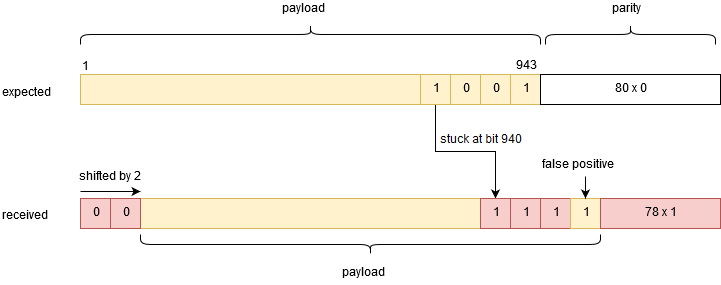
\includegraphics[width=0.65\textwidth]{figures/decoder_parity.png}
\caption{Response shift in the BCH Decoder tested much over it's max. frequency}
\label{fig:shift}
\end{figure}

In the normal operation the parity bits would be 0 and flipped only by Chien Search Block in case of error correction. Since the input data is manipulated only by one logic gate (LUT) during the correction and the $ISERR$ bit is not causing the correction, the error happens in the decoder interface. The design is isolated with additional flip-flops and direct output is always compared with the delayed output to detect the delay errors on the DOUT signal. The same applies for input signal. The routing tool decided however to place the delay registers far away from the decoder and close to the test engine. It makes the delayed path and direct path almost equally long and they fail at the same time, therefore the detection of the delay fault is not possible. The situation is presented in \autoref{subfig:uncon}.

\begin{figure}[h]
\centering
\begin{subfigure}{.45\textwidth}
    \centering
    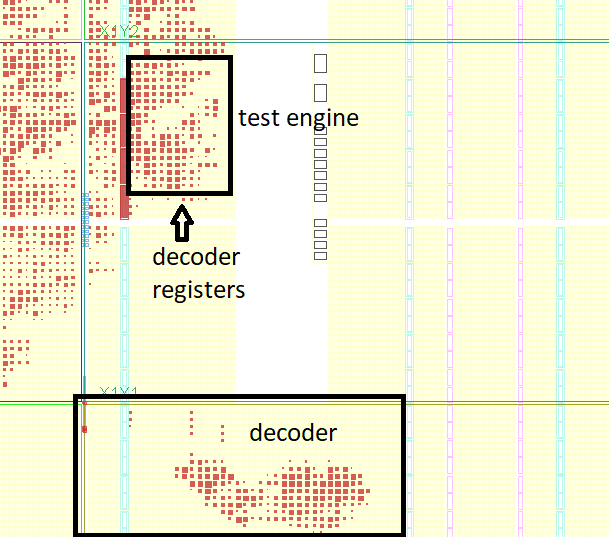
\includegraphics[width=\linewidth]{figures/Device_edited.png}
    \caption{Unconstrained}
    \label{subfig:uncon}
\end{subfigure}%
\hspace{\fill}
\begin{subfigure}{.45\textwidth}
    \centering
    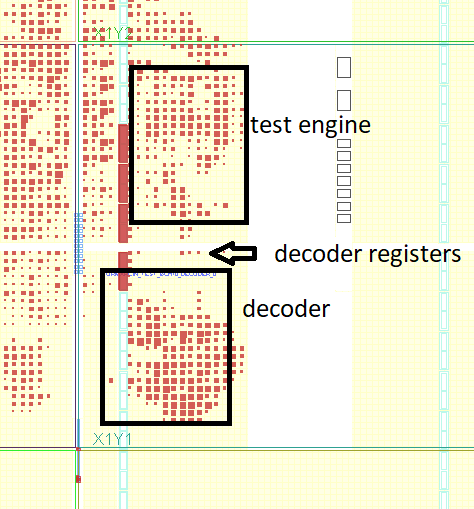
\includegraphics[width=\linewidth]{figures/Device_Pblock_edited.png}
    \caption{Constrained}
    \label{subfig:con}
\end{subfigure}
\caption{Decoder placement in FPGA}
\label{fig:dec_routing}
\end{figure}

In conclusion, the errors showing up by 300 MHz are due to long paths between the decoder and the test engine, having nothing to do with the internal structure of the decoder.

Failing interconnects lead to interesting conclusion, that the delay faults in the FPGA may be injected by exploiting the placing tools by positioning chosen cells apart from the main design, to guarantee that they will fail as first, when the frequency gets raised. It is important to remind, that the delay faults in real hardware may happen in other paths, not necessarily the longest ones.

Since the design can be influenced by constraining the placement tool, the further tests were conducted on a decoder enclosed in so called PBLOCK. The PBLOCKS are areas in the FPGA, that force the placement tool to try to fit parts of the design inside of them. After drawing the PBLOCK between the old decoder position and the test engine, the decoder was placed closer to the test engine, so the delay fault at the interconnect should appear later or the delayed and direct signal should differ. This situation in presented in \autoref{subfig:con}. The tests of constrained design showed that the maximal frequencies were different, because the distances between various cells were different. The design has been closed in smaller space, making the circuit more dense and the cells were repositioned. The maximal frequencies of the constrained design have been presented in \autoref{tab:dec}. The positions of errors did not change, only the frequency, when they started to appear. The delay fault on the interconnect doesn't appear until 365 MHz. This time the delay faults were detected thanks to the delay logic.

The placement of the design seems to have great impact on test results. The delay faults happening on the interface can be detected by delay logic and comparison, but the placement of this logic is also of grave importance. The decoder circuit is unable to detect more errors then it can correct. In case of permanent faults in the decoder, special BIST techniques need to be incorporated, since the faults will have influence on the results of the diagnostic test. The diagnostic test can show that the decoder or encoder is faulty. Since the encoder faults are expected to produce errors in parity bits and the decoder errors reside randomly in the whole code word, the position of the error should give good indication on which module failed. The additional internal test can be conducted with suggested method of testing the LFSRs \cite{art:Gleichner} or in regular decoder circuits, like Hsiao-Code decoders, using spare modules and glitch filters \cite{art:Dicorato}.


\chapter{Summary}

The diagnostic test is limited by the error detection capability of the decoder. The more errors a decoder can detect, the better chance of reliable test result. In systems with single error correction and double error detection (SEC-DEC), like those implementing extended Hamming-code or Hsiao-code, the common weak point is erroneous error detection in case of triple bit errors and multiple bit errors \cite{art:Dicorato}. The diagnostic test based on those modules may produce false positive results in such systems, assuming that single fault may corrupt more bits in the data bit stream. In communication systems, where data is processed serially, like in BCH encoder and decoder tested in this thesis, the occurrence of multiple bit flips in case of single fault is very high. In case of BCH decoders, it may require to redesign the architecture to implement the capabilities of underlaying ECC fully or in case of PENCA, which is a reconfigurable solution, to choose the code with highest correction capability, which is 15 bit errors in a single message \cite{art:Pfeifer}.

Another limitation to the diagnostic test solution is the coverage of only those modules, which lay between encoder and decoder. The source encoding and cryptographic encryption are only two examples of modules, that may reside outside of the test subsystem, not covered by the diagnostic test. For those modules, well established digital test methods need to be applied. The same restriction applies to the decoder architecture itself. It has been admittedly reported, that some decoder architectures, like Hsiao-code decoder are capable of correcting (masking) some of its own hardware faults happening in the embedded encoder structure, under condition that they don't overlap with the transmission errors \cite{art:Dicorato}, but this feature does not cover the entire decoder structure and lowers the error coverage of the deocder. In the BCH decoder if any syndrome is non-zero a correction is triggered, so any fault in syndrome generation unit, that leads to a failure of the unit, will trigger a false correction, therefore an error in output bit stream. The same applies to the Key Solver unit or Chien Search Block. In all cases, the diagnostic test doesn't cover the decoder internal faults so the decoder dependability needs to be taken care of separately. The diagnostic test can help in finding encoder or decoder faulty, since the last shortcut tests only those two modules. In case of failed test, as in all other cases, the repair of one unit is conducted and the test is repeated.

Moreover the diagnostic test is used only for error detection. The repair of permanent faults require further redundancy, like spare units, leading to duplication of the hardware or parts of it. In case of patent protected circuitry, with no additional DfT extensions, a full duplication of hardware seems to be the only way to ensure repair possibility. Thanks to the diagnostic test, there is no need for trippling the hardware to create a TMR system.

The additional multiplexers, laying on transmission path, lead to signal deterioration, which is especially important in the analog part. The multiplexers need to be adjusted, so that their response does not disturb "normal" functionality of the system. In digital logic, the additional multiplexers create additional delay, although the switching happens off-line, so it should not influence the "normal" function.

The suggested diagnostic test requires also control logic to conduct the "fake" start-up procedure and maybe run some additional test vectors through the design to detect faults not visible during the start-up phase. Most of it can reside in software, since the test uses "normal" data path. The only signals needed during the implementation were the $ISERR$ output of the decoder and control signals to enable shortcuts. To conduct the repair, additional control inputs need to be provided.

In conclusion, the suggested solution is useful as diagnostic test in systems with no internal access to some modules laying between FEC encoder and decoder and allows the test of analog, mixed-signal and digital modules indifferently with just little hardware and software overhead. The test is limited by error detection capability of the decoder. The limitation is not different then the test result evaluation using signatures. The tests are false positive in case of error vectors changing one code word into another valid code word, just like conflicts happening in signature calculation. To extend the test to all modules in transceiver and receiver, more shortcuts can be added, between all corresponding modules, and the response analysis may happen in the software. This approach may be triggered when the proposed diagnostic test fails its purpose.

The results of tests conducted on encoder and decoder architectures, helped by the development process and were a valuable input in understanding the limitations of the designs. They also validated the proper functionality of the basic PENCA building blocks and showed, in case of decoder, where are the possible bottlenecks. Unfortunately, the test engine was not successful in testing the limits of encoder architecture.

As a result of this thesis, a useful tool for design validation in "real" hardware was developed and may be used as an alternative to simulation, speeding up the development process and allowing quick evaluation of responses with any chosen program. The placement of the design is to be treated with much caution and understanding, to avoid misinterpretation of test results. 